%%  
%% TGARS Draft - JLG input 8/
%%bare_jrnl.tex
%% V1.4a
%% 2014/09/17
%% by Michael Shell
%% see http://www.michaelshell.org/
%% for current contact information.
%%
%% This is a skeleton file demonstrating the use of IEEEtran.cls
%% (requires IEEEtran.cls version 1.8a or later) with an IEEE
%% journal paper.
%%
%% Support sites:
%% http://www.michaelshell.org/tex/ieeetran/
%% http://www.ctan.org/tex-archive/macros/latex/contrib/IEEEtran/
%% and
%% http://www.ieee.org/

%%*************************************************************************
%% Legal Notice:
%% This code is offered as-is without any warranty either expressed or
%% implied; without even the implied warranty of MERCHANTABILITY or
%% FITNESS FOR A PARTICULAR PURPOSE! 
%% User assumes all risk.
%% In no event shall IEEE or any contributor to this code be liable for
%% any damages or losses, including, but not limited to, incidental,
%% consequential, or any other damages, resulting from the use or misuse
%% of any information contained here.
%%
%% All comments are the opinions of their respective authors and are not
%% necessarily endorsed by the IEEE.
%%
%% This work is distributed under the LaTeX Project Public License (LPPL)
%% ( http://www.latex-project.org/ ) version 1.3, and may be freely used,
%% distributed and modified. A copy of the LPPL, version 1.3, is included
%% in the base LaTeX documentation of all distributions of LaTeX released
%% 2003/12/01 or later.
%% Retain all contribution notices and credits.
%% ** Modified files should be clearly indicated as such, including  **
%% ** renaming them and changing author support contact information. **
%%
%% File list of work: IEEEtran.cls, IEEEtran_HOWTO.pdf, bare_adv.tex,
%%                    bare_conf.tex, bare_jrnl.tex, bare_conf_compsoc.tex,
%%                    bare_jrnl_compsoc.tex, bare_jrnl_transmag.tex
%%*************************************************************************


% *** Authors should verify (and, if needed, correct) their LaTeX system  ***
% *** with the testflow diagnostic prior to trusting their LaTeX platform ***
% *** with production work. IEEE's font choices and paper sizes can       ***
% *** trigger bugs that do not appear when using other class files.       ***                          ***
% The testflow support page is at:
% http://www.michaelshell.org/tex/testflow/



\documentclass[draftcls]{IEEEtran}
%
% If IEEEtran.cls has not been installed into the LaTeX system files,
% manually specify the path to it like:
% \documentclass[journal]{../sty/IEEEtran}





% Some very useful LaTeX packages include:
% (uncomment the ones you want to load)


% *** MISC UTILITY PACKAGES ***
%
%\usepackage{ifpdf}
% Heiko Oberdiek's ifpdf.sty is very useful if you need conditional
% compilation based on whether the output is pdf or dvi.
% usage:
% \ifpdf
%   % pdf code
% \else
%   % dvi code
% \fi
% The latest version of ifpdf.sty can be obtained from:
% http://www.ctan.org/tex-archive/macros/latex/contrib/oberdiek/
% Also, note that IEEEtran.cls V1.7 and later provides a builtin
% \ifCLASSINFOpdf conditional that works the same way.
% When switching from latex to pdflatex and vice-versa, the compiler may
% have to be run twice to clear warning/error messages.






% *** CITATION PACKAGES ***
%
%\usepackage{cite}
% cite.sty was written by Donald Arseneau
% V1.6 and later of IEEEtran pre-defines the format of the cite.sty package
% \cite{} output to follow that of IEEE. Loading the cite package will
% result in citation numbers being automatically sorted and properly
% "compressed/ranged". e.g., [1], [9], [2], [7], [5], [6] without using
% cite.sty will become [1], [2], [5]--[7], [9] using cite.sty. cite.sty's
% \cite will automatically add leading space, if needed. Use cite.sty's
% noadjust option (cite.sty V3.8 and later) if you want to turn this off
% such as if a citation ever needs to be enclosed in parenthesis.
% cite.sty is already installed on most LaTeX systems. Be sure and use
% version 5.0 (2009-03-20) and later if using hyperref.sty.
% The latest version can be obtained at:
% http://www.ctan.org/tex-archive/macros/latex/contrib/cite/
% The documentation is contained in the cite.sty file itself.






% *** GRAPHICS RELATED PACKAGES ***
%
\ifCLASSINFOpdf
   \usepackage[pdftex]{graphicx}
  % declare the path(s) where your graphic files are
   \graphicspath{{../pdf/}{../jpeg/}}
  % and their extensions so you won't have to specify these with
  % every instance of \includegraphics
   \DeclareGraphicsExtensions{.pdf,.jpeg,.png}
\else
  % or other class option (dvipsone, dvipdf, if not using dvips). graphicx
  % will default to the driver specified in the system graphics.cfg if no
  % driver is specified.
  % \usepackage[dvips]{graphicx}
  % declare the path(s) where your graphic files are
  % \graphicspath{{../eps/}}
  % and their extensions so you won't have to specify these with
  % every instance of \includegraphics
  % \DeclareGraphicsExtensions{.eps}
\fi
% graphicx was written by David Carlisle and Sebastian Rahtz. It is
% required if you want graphics, photos, etc. graphicx.sty is already
% installed on most LaTeX systems. The latest version and documentation
% can be obtained at: 
% http://www.ctan.org/tex-archive/macros/latex/required/graphics/
% Another good source of documentation is "Using Imported Graphics in
% LaTeX2e" by Keith Reckdahl which can be found at:
% http://www.ctan.org/tex-archive/info/epslatex/
%
% latex, and pdflatex in dvi mode, support graphics in encapsulated
% postscript (.eps) format. pdflatex in pdf mode supports graphics
% in .pdf, .jpeg, .png and .mps (metapost) formats. Users should ensure
% that all non-photo figures use a vector format (.eps, .pdf, .mps) and
% not a bitmapped formats (.jpeg, .png). IEEE frowns on bitmapped formats
% which can result in "jaggedy"/blurry rendering of lines and letters as
% well as large increases in file sizes.
%
% You can find documentation about the pdfTeX application at:
% http://www.tug.org/applications/pdftex





% *** MATH PACKAGES ***
%
\usepackage[cmex10]{amsmath}
% A popular package from the American Mathematical Society that provides
% many useful and powerful commands for dealing with mathematics. If using
% it, be sure to load this package with the cmex10 option to ensure that
% only type 1 fonts will utilized at all point sizes. Without this option,
% it is possible that some math symbols, particularly those within
% footnotes, will be rendered in bitmap form which will result in a
% document that can not be IEEE Xplore compliant!
%
% Also, note that the amsmath package sets \interdisplaylinepenalty to 10000
% thus preventing page breaks from occurring within multiline equations. Use:
%\interdisplaylinepenalty=2500
% after loading amsmath to restore such page breaks as IEEEtran.cls normally
% does. amsmath.sty is already installed on most LaTeX systems. The latest
% version and documentation can be obtained at:
% http://www.ctan.org/tex-archive/macros/latex/required/amslatex/math/





% *** SPECIALIZED LIST PACKAGES ***
%
\usepackage{algorithmic}
% algorithmic.sty was written by Peter Williams and Rogerio Brito.
% This package provides an algorithmic environment fo describing algorithms.
% You can use the algorithmic environment in-text or within a figure
% environment to provide for a floating algorithm. Do NOT use the algorithm
% floating environment provided by algorithm.sty (by the same authors) or
% algorithm2e.sty (by Christophe Fiorio) as IEEE does not use dedicated
% algorithm float types and packages that provide these will not provide
% correct IEEE style captions. The latest version and documentation of
% algorithmic.sty can be obtained at:
% http://www.ctan.org/tex-archive/macros/latex/contrib/algorithms/
% There is also a support site at:
% http://algorithms.berlios.de/index.html
% Also of interest may be the (relatively newer and more customizable)
% algorithmicx.sty package by Szasz Janos:
% http://www.ctan.org/tex-archive/macros/latex/contrib/algorithmicx/




% *** ALIGNMENT PACKAGES ***
%
\usepackage{array}
% Frank Mittelbach's and David Carlisle's array.sty patches and improves
% the standard LaTeX2e array and tabular environments to provide better
% appearance and additional user controls. As the default LaTeX2e table
% generation code is lacking to the point of almost being broken with
% respect to the quality of the end results, all users are strongly
% advised to use an enhanced (at the very least that provided by array.sty)
% set of table tools. array.sty is already installed on most systems. The
% latest version and documentation can be obtained at:
% http://www.ctan.org/tex-archive/macros/latex/required/tools/


% IEEEtran contains the IEEEeqnarray family of commands that can be used to
% generate multiline equations as well as matrices, tables, etc., of high
% quality.




% *** SUBFIGURE PACKAGES ***
%\ifCLASSOPTIONcompsoc
%  \usepackage[caption=false,font=normalsize,labelfont=sf,textfont=sf]{subfig}
%\else
%  \usepackage[caption=false,font=footnotesize]{subfig}
%\fi
% subfig.sty, written by Steven Douglas Cochran, is the modern replacement
% for subfigure.sty, the latter of which is no longer maintained and is
% incompatible with some LaTeX packages including fixltx2e. However,
% subfig.sty requires and automatically loads Axel Sommerfeldt's caption.sty
% which will override IEEEtran.cls' handling of captions and this will result
% in non-IEEE style figure/table captions. To prevent this problem, be sure
% and invoke subfig.sty's "caption=false" package option (available since
% subfig.sty version 1.3, 2005/06/28) as this is will preserve IEEEtran.cls
% handling of captions.
% Note that the Computer Society format requires a larger sans serif font
% than the serif footnote size font used in traditional IEEE formatting
% and thus the need to invoke different subfig.sty package options depending
% on whether compsoc mode has been enabled.
%
% The latest version and documentation of subfig.sty can be obtained at:
% http://www.ctan.org/tex-archive/macros/latex/contrib/subfig/




% *** FLOAT PACKAGES ***
%
%\usepackage{fixltx2e}
% fixltx2e, the successor to the earlier fix2col.sty, was written by
% Frank Mittelbach and David Carlisle. This package corrects a few problems
% in the LaTeX2e kernel, the most notable of which is that in current
% LaTeX2e releases, the ordering of single and double column floats is not
% guaranteed to be preserved. Thus, an unpatched LaTeX2e can allow a
% single column figure to be placed prior to an earlier double column
% figure. The latest version and documentation can be found at:
% http://www.ctan.org/tex-archive/macros/latex/base/


%\usepackage{stfloats}
% stfloats.sty was written by Sigitas Tolusis. This package gives LaTeX2e
% the ability to do double column floats at the bottom of the page as well
% as the top. (e.g., "\begin{figure*}[!b]" is not normally possible in
% LaTeX2e). It also provides a command:
%\fnbelowfloat
% to enable the placement of footnotes below bottom floats (the standard
% LaTeX2e kernel puts them above bottom floats). This is an invasive package
% which rewrites many portions of the LaTeX2e float routines. It may not work
% with other packages that modify the LaTeX2e float routines. The latest
% version and documentation can be obtained at:
% http://www.ctan.org/tex-archive/macros/latex/contrib/sttools/
% Do not use the stfloats baselinefloat ability as IEEE does not allow
% \baselineskip to stretch. Authors submitting work to the IEEE should note
% that IEEE rarely uses double column equations and that authors should try
% to avoid such use. Do not be tempted to use the cuted.sty or midfloat.sty
% packages (also by Sigitas Tolusis) as IEEE does not format its papers in
% such ways.
% Do not attempt to use stfloats with fixltx2e as they are incompatible.
% Instead, use Morten Hogholm'a dblfloatfix which combines the features
% of both fixltx2e and stfloats:
%
% \usepackage{dblfloatfix}
% The latest version can be found at:
% http://www.ctan.org/tex-archive/macros/latex/contrib/dblfloatfix/




%\ifCLASSOPTIONcaptionsoff
%  \usepackage[nomarkers]{endfloat}
% \let\MYoriglatexcaption\caption
% \renewcommand{\caption}[2][\relax]{\MYoriglatexcaption[#2]{#2}}
%\fi
% endfloat.sty was written by James Darrell McCauley, Jeff Goldberg and 
% Axel Sommerfeldt. This package may be useful when used in conjunction with 
% IEEEtran.cls'  captionsoff option. Some IEEE journals/societies require that
% submissions have lists of figures/tables at the end of the paper and that
% figures/tables without any captions are placed on a page by themselves at
% the end of the document. If needed, the draftcls IEEEtran class option or
% \CLASSINPUTbaselinestretch interface can be used to increase the line
% spacing as well. Be sure and use the nomarkers option of endfloat to
% prevent endfloat from "marking" where the figures would have been placed
% in the text. The two hack lines of code above are a slight modification of
% that suggested by in the endfloat docs (section 8.4.1) to ensure that
% the full captions always appear in the list of figures/tables - even if
% the user used the short optional argument of \caption[]{}.
% IEEE papers do not typically make use of \caption[]'s optional argument,
% so this should not be an issue. A similar trick can be used to disable
% captions of packages such as subfig.sty that lack options to turn off
% the subcaptions:
% For subfig.sty:
% \let\MYorigsubfloat\subfloat
% \renewcommand{\subfloat}[2][\relax]{\MYorigsubfloat[]{#2}}
% However, the above trick will not work if both optional arguments of
% the \subfloat command are used. Furthermore, there needs to be a
% description of each subfigure *somewhere* and endfloat does not add
% subfigure captions to its list of figures. Thus, the best approach is to
% avoid the use of subfigure captions (many IEEE journals avoid them anyway)
% and instead reference/explain all the subfigures within the main caption.
% The latest version of endfloat.sty and its documentation can obtained at:
% http://www.ctan.org/tex-archive/macros/latex/contrib/endfloat/
%
% The IEEEtran \ifCLASSOPTIONcaptionsoff conditional can also be used
% later in the document, say, to conditionally put the References on a 
% page by themselves.




% *** PDF, URL AND HYPERLINK PACKAGES ***
%
%\usepackage{url}
% url.sty was written by Donald Arseneau. It provides better support for
% handling and breaking URLs. url.sty is already installed on most LaTeX
% systems. The latest version and documentation can be obtained at:
% http://www.ctan.org/tex-archive/macros/latex/contrib/url/
% Basically, \url{my_url_here}.




% *** Do not adjust lengths that control margins, column widths, etc. ***
% *** Do not use packages that alter fonts (such as pslatex).         ***
% There should be no need to do such things with IEEEtran.cls V1.6 and later.
% (Unless specifically asked to do so by the journal or conference you plan
% to submit to, of course. )


% correct bad hyphenation here
\hyphenation{op-tical net-works semi-conduc-tor}


\begin{document}
%
% paper title
% Titles are generally capitalized except for words such as a, an, and, as,
% at, but, by, for, in, nor, of, on, or, the, to and up, which are usually
% not capitalized unless they are the first or last word of the title.
% Linebreaks \\ can be used within to get better formatting as desired.
% Do not put math or special symbols in the title.
\title{Sensitivity Analysis of Reflectivity Retrieval from P-band Signals of Opportunity Observations}
%
%
% author names and IEEE memberships
% note positions of commas and nonbreaking spaces ( ~ ) LaTeX will not break
% a structure at a ~ so this keeps an author's name from being broken across
% two lines.
% use \thanks{} to gain access to the first footnote area
% a separate \thanks must be used for each paragraph as LaTeX2e's \thanks
% was not built to handle multiple paragraphs
%

\author{Yao-Cheng~Lin,~\IEEEmembership{Member,~IEEE,}
        Georges~Stienne,~\IEEEmembership{Member,~IEEE,}
        and~James~Garrison,~\IEEEmembership{Fellow,~IEEE}% <-this % stops a space
\thanks{Yao-Cheng Lin is with Aeronautics and Astronautics, Purdue University, Indiana,
IN, 47907}}

% note the % following the last \IEEEmembership and also \thanks - 
% these prevent an unwanted space from occurring between the last author name
% and the end of the author line. i.e., if you had this:
% 
% \author{....lastname \thanks{...} \thanks{...} }
%                     ^------------^------------^----Do not want these spaces!
%
% a space would be appended to the last name and could cause every name on that
% line to be shifted left slightly. This is one of those "LaTeX things". For
% instance, "\textbf{A} \textbf{B}" will typeset as "A B" not "AB". To get
% "AB" then you have to do: "\textbf{A}\textbf{B}"
% \thanks is no different in this regard, so shield the last } of each \thanks
% that ends a line with a % and do not let a space in before the next \thanks.
% Spaces after \IEEEmembership other than the last one are OK (and needed) as
% you are supposed to have spaces between the names. For what it is worth,
% this is a minor point as most people would not even notice if the said evil
% space somehow managed to creep in.



% The paper headers
\markboth{Journal of \LaTeX\ Class Files,~Vol.~13, No.~9, September~2014}%
{Shell \MakeLowercase{\textit{et al.}}: Bare Demo of IEEEtran.cls for Journals}
% The only time the second header will appear is for the odd numbered pages
% after the title page when using the twoside option.
% 
% *** Note that you probably will NOT want to include the author's ***
% *** name in the headers of peer review papers.                   ***
% You can use \ifCLASSOPTIONpeerreview for conditional compilation here if
% you desire.




% If you want to put a publisher's ID mark on the page you can do it like
% this:
%\IEEEpubid{0000--0000/00\$00.00~\copyright~2014 IEEE}
% Remember, if you use this you must call \IEEEpubidadjcol in the second
% column for its text to clear the IEEEpubid mark.



% use for special paper notices
%\IEEEspecialpapernotice{(Invited Paper)}




% make the title area
\maketitle

% As a general rule, do not put math, special symbols or citations
% in the abstract or keywords.
\begin{abstract}
Signals of Opportunity Airborne Demonstrator (SoOp-AD) is a NASA Instrument Incubator Program (IIP-13) selection to demonstrate remote sensing of Root Zone Soil Moisture (RZSM) using P-band signals of opportunity (SoOp). Soil penetration depth at these frequencies is 10’s of cm. Three basic observations will be produced from this instrument: autocorrelation of the direct signal, autocorrelation of the reflected signal, and the complex cross-correlation between the direct and reflected signals. Two reflectivity estimates, the ratio of the auto-correlations and the ratio of cross- to auto-correlation, have been defined, allowing soil moisture to be retrieved using established empirical models for the soil dielectric constant. In P-band, the available satellite transmissions have very low bandwidth (individual 5-25 kHz channels). An aircraft antenna designed for this wavelength would have a very wide beamwidth. These considerations preclude relying upon delay or antenna beam to provide strong isolation between direct and reflected ray paths. Consequently, both the sky-view and Earth-view antennas would receive a combination of direct and reflected signals. Algorithms for the retrieval of reflectivity, and thus RZSM, from observations of these signals must incorporate an understanding of this interference. Using synthetic signals having realistic noise power, a calibration function is developed to correct these observable s, accounting for the cross-channel interference. A sensitivity study was conducted, to evaluate the dependence of retrieval accuracy on the uncertainty in antenna gain pattern, aircraft attitude, and receiver calibration. These simulation studies, conducted over an ensemble of expected soil moisture, were used to define system requirements meeting the science requirement to retrieve volumetric soil moisture with a root mean square error of less than 0.04.
\end{abstract}

% Note that keywords are not normally used for peerreview papers.
\begin{IEEEkeywords}
Remote sensing, Signal of opportunity, soil moisture, P-band.
\end{IEEEkeywords}


% For peer review papers, you can put extra information on the cover
% page as needed:
% \ifCLASSOPTIONpeerreview
% \begin{center} \bfseries EDICS Category: 3-BBND \end{center}
% \fi
%
% For peerreview papers, this IEEEtran command inserts a page break and
% creates the second title. It will be ignored for other modes.
\IEEEpeerreviewmaketitle

\section{Introduction}
% The very first letter is a 2 line initial drop letter followed
% by the rest of the first word in caps.
% 
% form to use if the first word consists of a single letter:
% \IEEEPARstart{A}{demo} file is ....
% 
% form to use if you need the single drop letter followed by
% normal text (unknown if ever used by IEEE):
% \IEEEPARstart{A}{}demo file is ....
% 
% Some journals put the first two words in caps:
% \IEEEPARstart{T}{his demo} file is ....
% 
% Here we have the typical use of a "T" for an initial drop letter
% and "HIS" in caps to complete the first word.
\IEEEPARstart{T}{he}measurement of soil moisture plays an important role in studying Earth's hydrosphere. Soil moisture is measured directly in situ at specific locations, however, the measurement in the region is not comprehensive for global studies because soil moisture highly depends on spatial distribution \cite{Wang:2009}. Satellite remote sensing provides several techniques for estimating soil moisture over a wide area, especially passive microwave radiometry is the most mature technology for the remote sensing of soil moisture. In 2009, ESA (European Space Agency) launched the SMOS (Soil Moisture and Ocean Salinity) satellite providing global maps of soil moisture and ocean salinity \cite{Kerr:2000}. Then the upcoming Soil Moisture Active Passive (SMAP) mission from National Aeronautics and Space Administration (NASA) \cite{Entekhabi:2010} will make global measurements of the soil moisture present at the Earth's land surface and will distinguish frozen from thawed land . However, the frequencies used in SMOS and SMAP are in L-band (1.4GHz) (the corresponding wavelength is about 21 cm) because of the required antenna size. Moreover, the specific frequency (1.4GHz) selected for SMOS and SMAP lies in a band protected for radio astronomy and thus utilizes strong isolation from radio frequency interference (RFI). The sensing depth for these frequencies, however, is limited to the first few centimeters of the soil.

Satellite remote sensing is not only limited in the observation of specific satellites, but Global Navigation Satellite System-Reflectometry (GNSS-R) has been demonstrated as an alternative approach to the remote sensing of soil moisture, through several airborne and ground-based experiments \cite{Zavorotny:2010} \cite{Larson:2008}. GNSS-R is a bistatic radar configuration, using the existing GNSS signals as the illumination source, producing a measurement of surface reflectivity, Γ, that is directly related to emissivity, ε, through conservation of energy; Γ=1-ε. GNSS-R thus provides a measurement of the exact physical property sensed by microwave radiometry, but with a substantially higher power due to the forward-scatter geometry and an active transmitter. This could enable a satellite receiver with a much smaller antenna, as compared to a radar or radiometer, to be used for soil moisture sensing. GNSS signals are designed with strong anti-jamming capabilities, a feature that should translate into a high RFI resistance for GNSS-R measurements, as compared to passive microwave radiometry. GNSS-R measurements from satellite would provide global coverage as a result of the GNSS constellation design. GNSS, however, is also an L-band system (1575.42 MHz) and thus, the observed depth of soil moisture would not be an improvement over that provided by L-band radiometry (a few cm).

To observe the soil moisture of different depths, the signals with various frequencies are necessary. Reflectometry, using these so-called "Signals of Opportunity", or SoOp, could potentially make these measurements with instrumentation that is an order of magnitude smaller and with lower power requirement than active SAR or passive radiometry. As with GNSS-R, the "process-gain" obtained through cross-correlating the reflected signal may also provide a stronger isolation from RFI. Such measurements have never been demonstrated before. The cross-correlation technique developed for GNSS-R was recently demonstrated on communication satellite signals. An important finding was that the higher SNR, and nearly random data modulation, of communications signals allowed cross-correlation to be performed between the direct and reflected signals, without the need for a model signal. In that experiment, ocean reflections from the two geostationary satellites providing the XM radio service were inverted to estimate the surface wind speed during a flight off the Chesapeake Bay \cite{Shah:2011}. According to successful demonstration to show reflectometry using any communication satellite signal with sufficient SNR and a nearly random modulation, the similar technology is applied to the other satellites such as UHF-follow On (UFO) satellites with frequency from 240 to 270 MHz.


% You must have at least 2 lines in the paragraph with the drop letter
% (should never be an issue)

% needed in second column of first page if using \IEEEpubid
%\IEEEpubidadjcol

\subsection{P-Band UHF-Follow On Satellites}
The Ultra High Frequency Follow-On (UFO) system is a communication satellite system whose function is to provide communications for airborne, ship, submarine and ground forces. UFO satellite system is a DOD sponsored program and operated by U.S. Navy. By now there are totally 11 satellites. The first launch is in Mar.1993 and the planned lifetime of UFO system is 14 years. It replaced FLTSATCOM and is scheduled to be replaced by MUOS. The orbit of UFO is geosynchronous orbit and the altitude is 32810 km. From F-1 to F-7, UFO satellites provide redundant command and ranging capabilities when the satellite is on station. The bandwidth of each satellite is 25 kHz and it is on board processing. According to the amateur radio website \cite{Matt:2014}, the frequencies from both satellites are as the following table. Table\ref{Table Band Plan} indicates the location for band plan for UFO satellites.

\begin{table}[ht]
\centering
\begin{tabular}  {|c|c|c|c|c|}
	\hline
     \textbf{Band Plan} & \textbf{November}	& \textbf{Quebec} &	\textbf{Papa} & \textbf{Oscar} \\
    \hline
    Name & UFO F5 & UFO F6 & UFO F7 & UFO F2 \\
    \hline
     Location &	105.6° W & 99.2° W & 	22.0° W	&  28.7° E\\
    \hline
    Name & UFO F11 & UFO F10 & UFO F9  & UFO F3 \\
    \hline
    Location& 71.1° E &	72.6° E &	135.0° E &	156.4° W \\
    \hline
\end{tabular}
\caption{The location and band plan of UFO satellites}
\label{Table Band Plan}
\end{table}

\subsection{Global Navigation Satellite System  Reflectometry (GNSS+R)}

GNSS-R is a bistatic radar configuration, using the existing GNSS signals as the illumination source, producing a measurement of surface reflectivity, $\Gamma$, that is directly related to emissivity, $\epsilon$, through conservation of energy; $ \Gamma = 1 - \epsilon $ \cite{Jin:2011}. GNSS-R thus provides a measurement of the exact physical property sensed by microwave radiometry, but with a substantially higher power due to the forward-scatter geometry and an active transmitter. This could enable a satellite receiver with a much smaller antenna, as compared to a radar or radiometer, to be used for soil moisture sensing. GNSS signals are designed with strong anti-jamming capabilities, a feature that should translate into a high RFI resistance for GNSS-R measurements, as compared to passive microwave radiometry. GNSS-R measurements from satellite would provide global coverage as a result of the GNSS constellation design. GNSS, however, is also an L-band system (1575.42 MHz) and thus, the observed depth of soil moisture would not be an improvement over that provided by L-band
radiometry (a few cm). The unique contribution of the research defined in this proposal would extend the penetration depth of soil moisture measurements by applying the GNSS-R technique to communication satellite signals at lower frequencies.

\subsection{Fresnel reflection}
Figure \ref{fig:Fresnel zone} indicates the Fresnel zone with specular point. The Fresnel zone can be calculated by
\begin{equation}
	F_n=\sqrt{n \lambda \frac{D_{TS}D_{RS}}{D_{TS}+D_{RS}}} \label{Eq: Fresnel_zone}
\end{equation}
Where $n$ is nth Fresnel zone, $\lambda$ is the wavelength of signal, $D_{TS}$ is the distance between the transmitter and specular point, $D_{RS}$ is the distance between the receiver and specular point. Because $D_{TS}$ is extremely large than $D_{RS}$, the equation can be re-written as,
\begin{equation}
	F_n=\sqrt{n \lambda D_{RS}} \Rightarrow F_n=\sqrt{\frac{\lambda h}{sin\theta} } \label{Eq: Fresnel_zone_reduce}
\end{equation}
Where $h$ is the height and $\theta$ is the elevation angle.
\begin{figure}[!t]
	\centering
	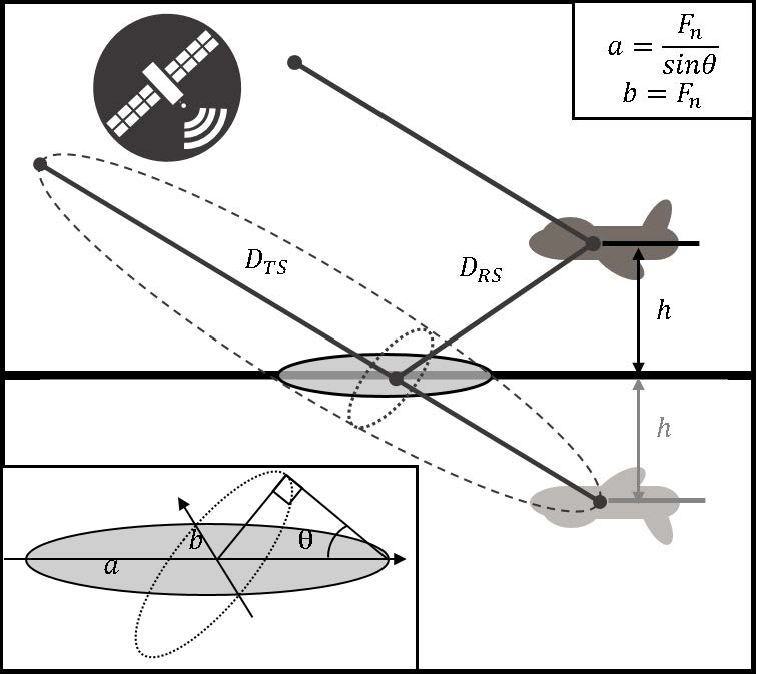
\includegraphics[width=2.5in]{pdf/Fresnel_zone.pdf}
	\caption{Fresnel zone for the specular point.}
    \centering
	\label{fig:Fresnel zone}
\end{figure}

\section{Soil moisture and reflectivity}
Dielectric constant of soil is a function Reflectivity is estimated by the measurement of SoOp, and the soil Dielectric constant is a very import factor for studying the reflectivity. The dielectric constant of media depends on the properties of media, for example, the dielectric constant of water can be calculated by temperature, salinity, and frequency.
\section{Reflectivity}

Reflectivity $\Gamma$ is the fraction of incident electromagnetic power that is reflected at an interface. The reflectivity can be represented by Fresnel refection coefficients $\mathcal{R}$.

\begin{equation}
\Gamma = |\mathcal{R}|^2=\frac{P_D}{P_R}
\end{equation}

Where $P_D$ and $P_R$ are the power of direct signal and reflection, respectively. $\mathcal{R}_{hh}$ and $\mathcal{R}_{vv}$ are the co-polar refection coefficients of horizontal plane $(h)$ and vertical plane $(v)$, and they can be expressed as

\begin{equation} 
\begin{split}
	{\mathcal{R}_{hh}} = {}& \frac{{{{\tilde \varepsilon }_r}\cos \theta  - \sqrt 				{{{\tilde \varepsilon }_r} - {{\sin }^2}\theta } }}{{{{\tilde \varepsilon}_r}				\cos \theta  + \sqrt {{{\tilde \varepsilon }_r} - {{\sin }^2}\theta }}}
\\
	{\mathcal{R}_{vv}} = {}& \frac{{\cos \theta  - \sqrt {{{\tilde \varepsilon }_r} - {{\sin }^2}\theta } }}{{\cos \theta  + \sqrt {{{\tilde \varepsilon }_r} - {{\sin }^2}\theta }}} 
    \end{split}
     \label{Eq: reflectivity_di}
\end{equation}

Where $\tilde{\varepsilon}_r$ is the complex relative complex dielectric constant  $\theta$ is the incident angle of signal. The circular polarization cab be transformed by the linear polarization. The transition matrix $\mathcal{T}$ is

\begin{equation*}
	\begin{matrix}
	\hat{u}_{r} = \frac{1}{\sqrt{2}}(\hat{u}_h - j\cdot \hat{u}_v) \\
	\hat{u}_{l} = \frac{1}{\sqrt{2}}(\hat{u}_h + j\cdot \hat{u}_v)
	\end{matrix}
	\Rightarrow 
	\begin{bmatrix}
	\hat{u}_{r} \\
	\hat{u}_{l}
	\end{bmatrix}= \frac{1}{\sqrt{2}}	 
	\begin{bmatrix}
	1 & -j \\
	1 & j
	\end{bmatrix}	
	\begin{bmatrix}
	\hat{u}_{h} \\
	\hat{u}_{v}
	\end{bmatrix}
\end{equation*}

\begin{equation}
	\mathcal{T}_{rl \rightarrow hv} =  \frac{1}{\sqrt{2}}	
	\begin{bmatrix}
	1 & -j \\
	1 & j
	\end{bmatrix}
\end{equation}

The coordinate of co-plane and cross plane for linear polarization and  can be transited to circular polarization by
\begin{equation}
 	\begin{bmatrix}
	\hat{u}_{r}\hat{u}_{r} & \hat{u}_{r}\hat{u}_{l} \\
	\hat{u}_{l}\hat{u}_{r} & \hat{u}_{l}\hat{u}_{l}
	\end{bmatrix} = 
	\begin{bmatrix}
	\hat{u}_{r} \\
	\hat{u}_{l} 
	\end{bmatrix}
	\begin{bmatrix}
	\hat{u}_{r} \\
	\hat{u}_{l} 
	\end{bmatrix}^* = 
	\mathcal{T}_{rl \rightarrow hv}
	\begin{bmatrix}
	\hat{u}_{h}\hat{u}_{h} & \hat{u}_{h}\hat{u}_{v} \\
	\hat{u}_{v}\hat{u}_{h} & \hat{u}_{v}\hat{u}_{v}
	\end{bmatrix}
	\mathcal{T}_{rl \rightarrow hv}^*
\end{equation}

Where $\hat{u}$ is the coordinate, the subscripts $h$ and $v$ represent the horizontal and vertical plane, and the subscripts $r$ and $l$ represent the RHCP and LHCP plane. Then the Fresnel reflection coefficients of the circular polarization are

\begin{equation}
	\begin{bmatrix}
	\mathcal{R}_{rr} & \mathcal{R}_{rl} \\
	\mathcal{R}_{lr} & \mathcal{R}_{ll}
	\end{bmatrix} = 
	\frac{1}{2}
	\begin{bmatrix}
	\mathcal{R}_{hh} + \mathcal{R}_{vv} & \mathcal{R}_{hh} - \mathcal{R}_{vv} \\
	\mathcal{R}_{hh} - \mathcal{R}_{vv} & \mathcal{R}_{hh} + \mathcal{R}_{vv}		\end{bmatrix}
\end{equation}




% Note that the IEEE does not put floats in the very first column
% - or typically anywhere on the first page for that matter. Also,
% in-text middle ("here") positioning is typically not used, but it
% is allowed and encouraged for Computer Society conferences (but
% not Computer Society journals). Most IEEE journals/conferences use
% top floats exclusively. 
% Note that, LaTeX2e, unlike IEEE journals/conferences, places
% footnotes above bottom floats. This can be corrected via the
% \fnbelowfloat command of the stfloats package.

\section{Dielectric constant of the soil}
\label{sec:DC_soil}
Dieletric constant of soil mixture depends on the frequency, temperature, salinity of soil, the bulk soil density, and soil moisture \cite{Peplinski:1995,Peplinski_correct:1995}.

\begin{equation} \label{eq: soil_dielectric_main}
\begin{split}
		 { \varepsilon_{soil} } &=  { \varepsilon'_{soil} } -j { \varepsilon''_{soil} } \\
    	 { \varepsilon'_{soil} } &= [1 + \frac{\rho_b}{\rho_{ss}} ( {\varepsilon_{s}^{\alpha}}-1) + (m_v^{\beta'}\varepsilon_{fw}^{\prime\alpha}-m_v]^{1/\alpha} \\
         { \varepsilon''_{soil} } &=m_v^{\beta"}\varepsilon_{fw}^{''\alpha}
\end{split}
\end{equation}

Where $\varepsilon_{soil}$ is the dielectric constant of soil, $\rho_b$ is the bulk density, $\rho_{ss}$ is the density of the solid soil material, $\varepsilon'_{fw}$ and $\varepsilon''_{fw}$ are the real and imaginary part of the dielectric constant of the free water, and $\alpha=0.65$ and $\beta$ are adjustable parameters. The adjustable parameters $\beta$ is a function of soil texture as follows,

\begin{equation}
\begin{split}
	\beta' &= 1.2748-0.519Soil_{sand}-0.152Soil_{clay} \\
    \beta'' &=1.33797-0.603Soil_{sand}-0.166Soil_{clay}
 \end{split}
\end{equation}
where $S$ and $C$ represent the mass fractions of sand and clay, respectively. The bulk density is also a function of soil texture \cite{Saxton:1986}.

\begin{equation} \label{eq: bulk_density}
\begin{split}
	 \rho_b &= (1-\Psi)\rho_b \\
	  \Psi &= 0.332 - 7.251 \cdot 10^{-4} Soil_{sand} + 0.1276 log_{10}(Soil_{clay})
\end{split}
\end{equation}

$\varepsilon_{s} $ is the dielectric constant of the solid soil is given by
\begin{equation}
	\varepsilon_s = (1.01+0.44\rho_s)^2-0.062
\end{equation}
The dielectric constant of free water $\varepsilon'_{fw}$ and $\varepsilon''_{fw}$ are expressed as the follows,
\begin{equation}
\begin{split}
	\varepsilon'_{fw} &=\varepsilon_{w\infty} + \frac{\varepsilon_{w0}-\varepsilon_{w\infty}}{1+(2 \pi f \tau_w)^2} \\
    \varepsilon''_{fw} &=\frac{2 \pi f \tau_w(\varepsilon_{w0}-\varepsilon_{w\infty})}{1+(2 \pi f \tau_w)^2} + \frac{\sigma_{eff}}{2 \pi \varepsilon_0 f} \frac{\rho_s-\rho_b}{\rho_s m_v} 
\end{split}
\end{equation}
where $\varepsilon_0$ is the permittivity of free space, $\tau_w$ represents the relaxation time for water, $f$ is the frequency in Hz, $\varepsilon_{w\infty}$ = 4.9 is the high-frequency limit of $\varepsilon'_{fw}$, and $m_v$ is the Volumetric soil moisture. The effective conductivity $\sigma_{eff}$ can be estimated as
\begin{equation}
	\sigma_{eff} = 0.0467+0.2204\rho_b-0.4111Soil_{sand}+0.6614Soil_{clay}
\end{equation}
Penetration depth is the decay of electromagnetic waves inside a material, and power of the field decays to $\frac{1}{e}$ of its surface value \cite{Ulaby:1981} . The penetration depth is given by
\begin{eqnarray}
	\alpha &&= \frac{2\pi}{\lambda} Im(\sqrt{\varepsilon_{soil}}) \\
    \delta_p &&= \frac{\alpha}{2}
\end{eqnarray}
Where  $\alpha$ attenuation constant.

\section{Soil moisture retrieval from reflectivity}
The dielectric constant of soil depends on the soil moisture in Equation \ref{eq: soil_dielectric_main} and the reflectivity is a function of the dielectric constant in Equation \ref{Eq: reflectivity_di}. Therefore, the relationship between the soil moisture and reflectivity can be established as shown in the top figure of  Figure \ref{fig:reflect_mv} when the soil texture, frequency, and salinity are known. The reflectivity of the same polarization is neglect since it is relatively small than the one of reverse polarization. The bottom figure of Figure \ref{fig:reflect_mv} is the inverse of the top figure, and the polynomial fit is used to retrieve soil moisture from reflectivity.

\begin{figure}[t!]
	\centering
	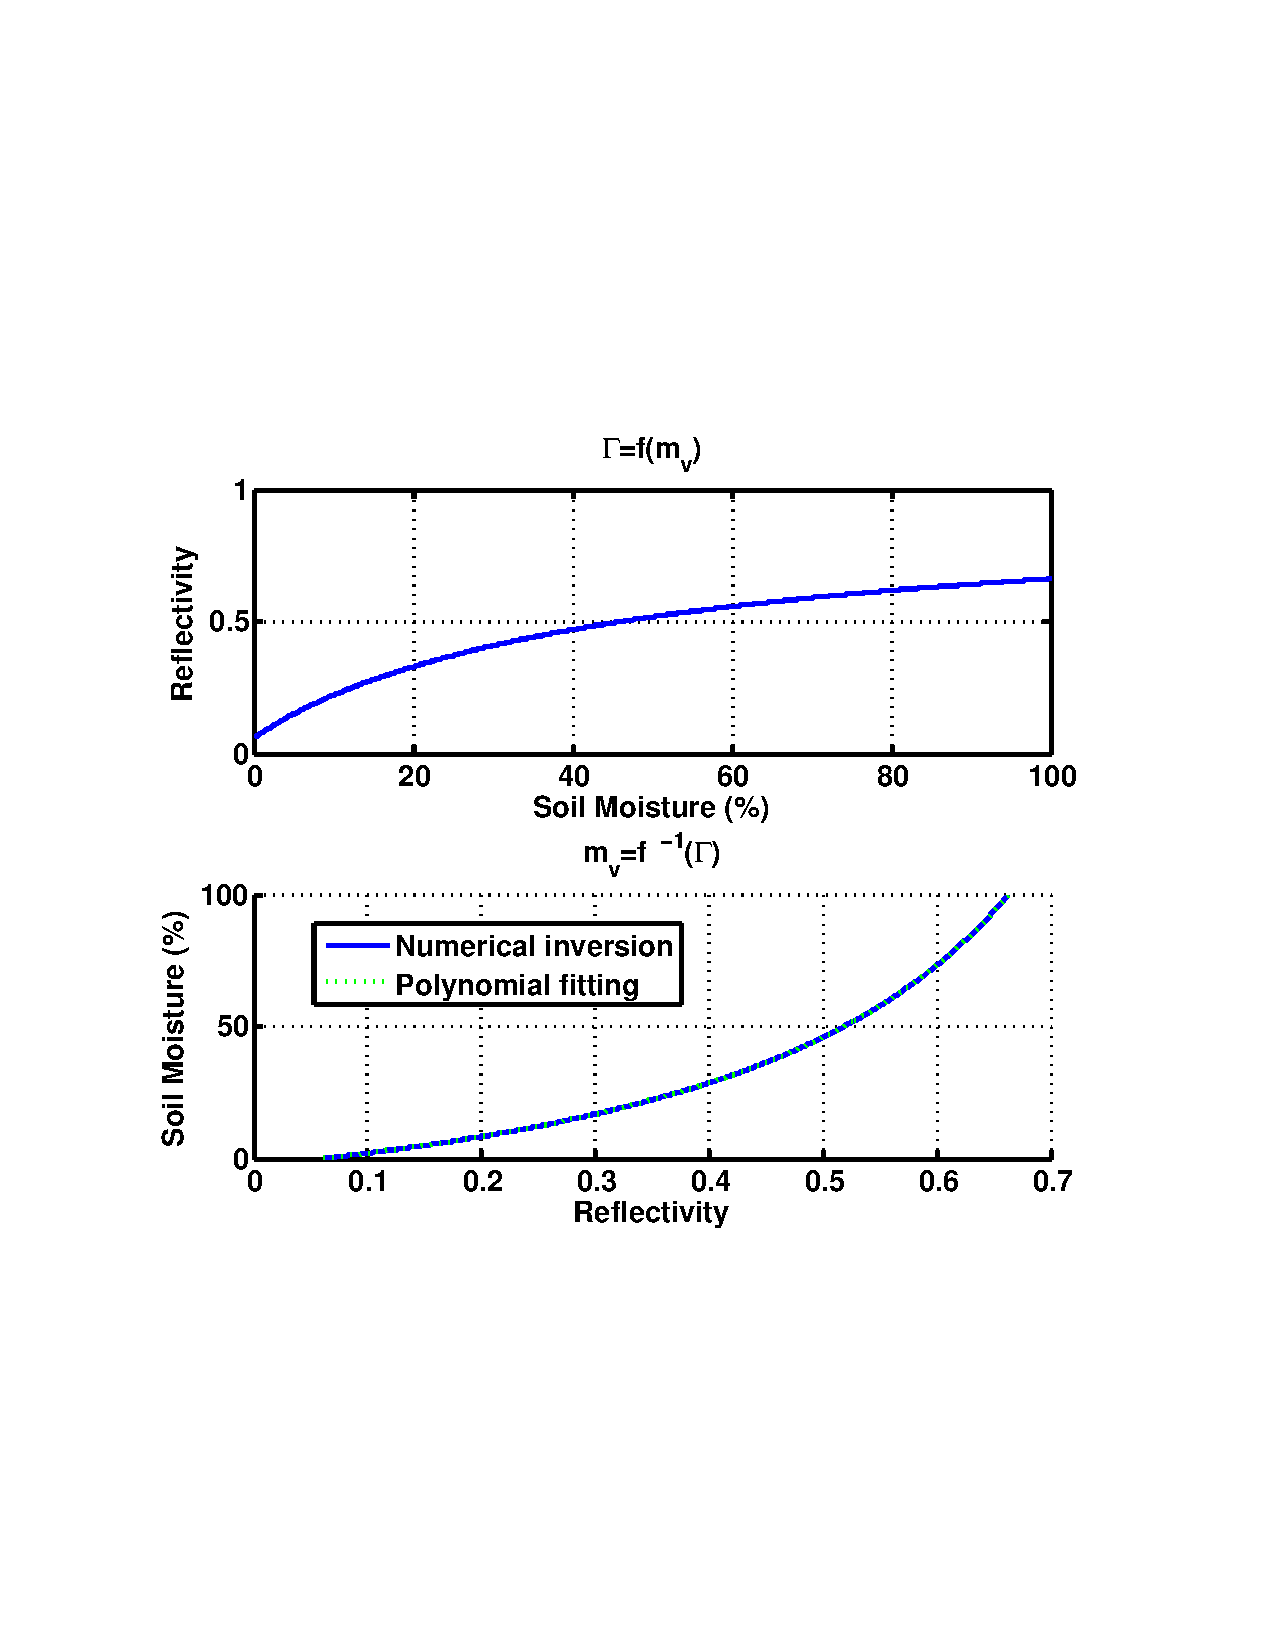
\includegraphics[width=4in]{pdf/gamma_vs_mv1.pdf}
	\caption{The reflectivity vs. soil moisture ($\%$) for the circular polarization}
	\centering
	\label{fig:reflect_mv}
\end{figure}
 The coefficients of a polynomial $P(x)$ of degree $N$ is given by
 \begin{equation}
	P(1)x^N+P(2)x^{N-1}+\cdots+P(N)x+P(N+1)
\end{equation} The coefficients of a polynomials in Figure \ref{fig:mv_reflect} are lists in Table \ref{Table:Polynomial_fitting}

\begin{table}[ht]
\centering
\begin{tabular}  {|c|c|c|c|c|c|}
	\hline
     Polynomial &1&2 &3&4&5\\
    \hline
   P-Band & 372.81 & -1200.41 &	1709.41 & -1390.75 & 710.29\\
     \hline
     Polynomial &6&7&8&9 &10\\
    \hline
   P-Band & -232.89 &	49.53 &	-5.68 & 0.84 & -0.04 \\
    \hline
\end{tabular}
\caption{The coefficients of a polynomial of degree 9}
\label{Table:Polynomial_fitting}
\end{table}

\section{Signal and correlation model}
The transmitted signal from a satellite ($x_{T}$) is modeled as
\begin{equation}
	x_T(t)=\sqrt{C_T}a(t)e^{j\omega_et},
    \label{Eq: xT}
\end{equation}
where the transmitted carrier power is $C_{T}$, $a(t)$ is the modulation, $ω_{e}$ is the free space frequency. The received signals at the object with antenna along the direct and reflected path ray can be represented \begin{equation}
	\begin{split}
  	x_D(t)&=\sqrt{C_D}a(t-\tau_D)e^{j\omega_e(t-\tau_D)}, \\
    x_R(t)&=\sqrt{C_R}a(t-\tau_R)e^{j\omega_e(t-\tau_R)}, 
    \end{split}
    \label{Eq: xD_xR}
\end{equation}
where $C_D$ and $C_R$ are received power of signals along direct and reflected path, and $\tau_D$ and $\tau_R$ are the path delay along the direct and reflected path. The reflectivity $\Gamma$ is defined as
\begin{equation}
	\Gamma=\frac{C_R}{C_D}
    \label{Eq: reflect}
\end{equation}
 After the receiver receives the signals, the models of signal for channel 1 and 2 are given by
 \begin{equation}
  \begin{split}
  	x_1(t)&=\sqrt{G_1}(\sqrt{G_{S,D}} x_D(t)) + \sqrt{G_{S,R}} x_R(t) + n_1)e^{-j\hat{\omega}_et},\\
    x_2(t)&=\sqrt{G_2}(\sqrt{G_{E,D}} x_D(t)) + \sqrt{G_{E,R}} x_R(t) + n_2)e^{-j\hat{\omega}_et},
  \end{split}
  \label{Eq: x1_x2_model}
\end{equation}
where $G$ is the gain in power ratio, $n$ is the noise with zero-mean, Gaussian, thermal noise with power spectra $\sigma^2_1$ and $\sigma^2_2$, and $\hat{\omega}_e$ is the down-convert frequency; the subscript $1$ and $2$ represent channel 1 and 2, and the subscript $S$ and $E$ denote the sky-view and earth-view antenna. Figure \ref{fig:ant_gain} shows the gain of sky-view and earth-view antenna along the direct and reflect paths.
\begin{figure}[t!]
	\centering
	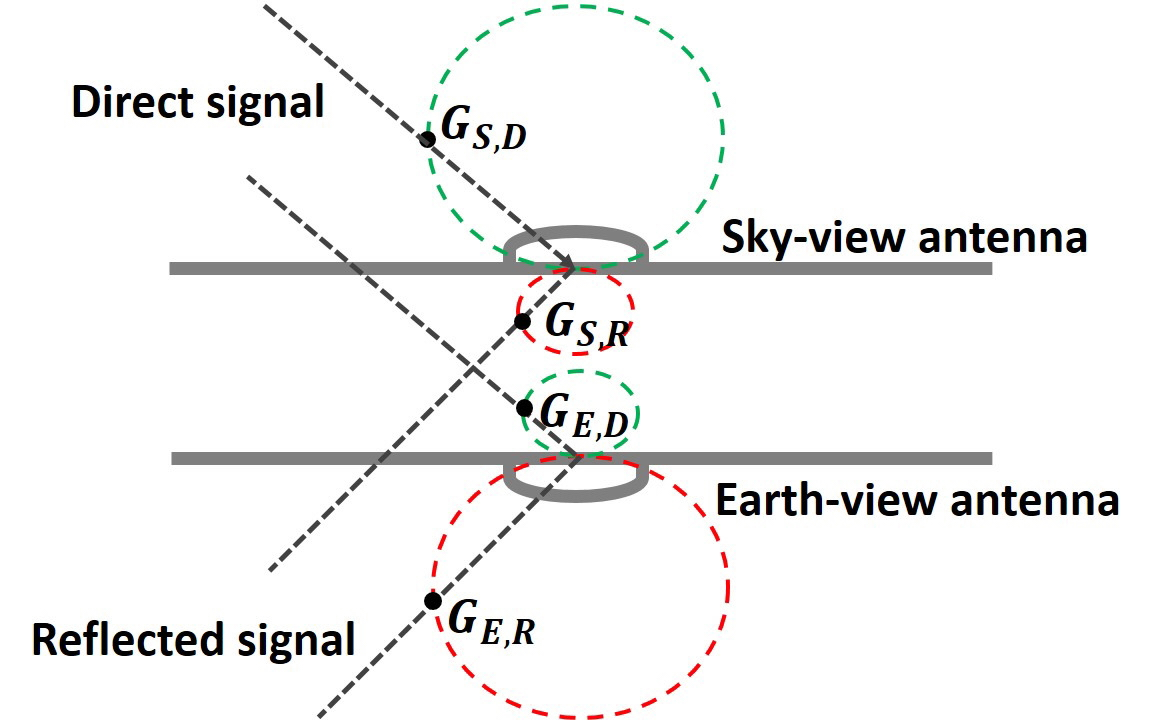
\includegraphics[width=2.5in]{pdf/ant_gain.jpg}
	\caption{The gain of sky-view and earth-view antenna for the direct and reflected path rays..}
	\centering
	\label{fig:ant_gain}
\end{figure}

\section{Correlation}

The correlation of two signals ($x_p$ and $x_q$) is defined as
\begin{eqnarray}
	R_{pq}(\tau)  = \langle x_p^*(t)x_q(t+\tau)\rangle=\frac{1}{T_I} \int_{T_I}x_p^*(t) x_q(t+\tau)dt \\ 
    R_{pq}(\tau-\tau_{qp}) =\langle x_p^*(t-\tau_p)x_q(t-\tau_q +\tau)\rangle
    \label{Eq: correlation_def}
\end{eqnarray}
Where $\tau_{qp}$ is the difference between the delay of $x_p$ and $x_q$, and $T_I$ is the integration time. The correlation $R_a(\tau)$ of $a(t)$, $a(t-\tau_D)$, and $a(t-\tau_R)$ are expressed as
\begin{equation}
\begin{split}
	R_a(\tau)&=\langle a^*(t)a(t +\tau)\rangle \\
    R_a(\tau-\tau_{RD})&=\langle a^*(t-\tau_D)a(t -\tau_R+\tau)\rangle \\
    R_a(\tau+\tau_{RD})&=\langle a^*(t-\tau_R)a(t -\tau_D+\tau)\rangle \\
 \end{split}
\end{equation}

The correlation of noise $n_1$ and $n_2$ are defined as
\begin{equation}
\begin{split}
	\langle n_1^*(t)n_1(t +\tau)\rangle &\approx \sigma^2_1 (\delta(\tau) +\tilde{n})\\
    \langle n_2^*(t)n_2(t +\tau)\rangle &\approx \sigma^2_2 (\delta(\tau) +\tilde{n})\\
    \langle n_1^*(t)n_2(t +\tau)\rangle &\approx \sigma_1 \sigma_2 \tilde{n}
 \end{split}
\end{equation}
In which
	
\[ \delta(\tau) = \left\{ 
  \begin{array}{l l}
    1 & \quad \text{if $\tau=0$}\\
    0 & \quad \text{else}
  \end{array} \right.\]

$\tilde{n}$ is the residual with zero mean. The auto-correlation $R_{11}$of $x_1$, auto-correlation $R_{22}$ of $x_2$, and cross-correlation $R_{12}$ of $x_1$ and $x_2$ can be derived by substituting Equation \ref{Eq: x1_x2_model} into Equation \ref{Eq: correlation_def}.
\begin{equation}
\begin{split}
	R_{11}(\tau^s) = (&g^2_{1SD} + g^2_{1SR})R_a(\tau^s)e^{j\Delta\omega_e\tau_s}+\\
    								 & g_{1SD} g_{1SR} (R_a(\tau^s-\tau^s_{RD})e^{j\omega_e \tau_{RD}}+\\ &R_a(\tau^s+\tau^s_{RD})e^{-j\omega_e \tau_{RD}})e^{-j\Delta\omega_e\tau_s}+\\
&G_1\sigma^2_1(\delta(\tau^s) + \tilde{n})                                     
\end{split}
\label{Eq: R11}
\end{equation}
\begin{equation}
\begin{split}
	R_{22}(\tau^s) = (&g^2_{2ED} + g^2_{2ER})R_a(\tau^s)e^{j\Delta\omega_e\tau_s}+\\
    								 & g_{2ED} g_{2ER} (R_a(\tau^s-\tau^s_{RD})e^{j\omega_e \tau_{RD}}+\\ &R_a(\tau^s+\tau^s_{RD})e^{-j\omega_e \tau_{RD}})e^{-j\Delta\omega_e\tau_s}+\\
&G_2\sigma^2_2(\delta(\tau^s) + \tilde{n})                                     
\end{split}
\label{Eq: R22}
\end{equation}
\begin{equation}
\begin{split}
	R_{12}(\tau^s) = (&g_{1SD} g_{2ED} + g_{1SR} g_{2ER})R_a(\tau^s)e^{j\Delta\omega_e\tau_s}+\\
    								 (& g_{1SD} g_{2ER} R_a(\tau^s-\tau^s_{RD})e^{j\omega_e \tau_{RD}}+\\ &g_{1SR} g_{2ED} R_a(\tau^s+\tau^s_{RD})e^{-j\omega_e \tau_{RD}})e^{j\Delta\omega_e\tau_s}+\\
&\sqrt{G_1 G_2}\sigma_1 \sigma_2 \tilde{n}                                     
\end{split}
\label{Eq: R12}
\end{equation}Where $\Delta \omega_e = \omega_e - \hat{\omega_e}$, $\tau^s$ are the samples, and 
\begin{eqnarray}
	g_{1SD} &= \sqrt{G_1 G_{S,D} C_D} \\
    g_{1SR} &= \sqrt{G_1 G_{S,R} C_R} \\
    g_{2ED} &= \sqrt{G_2 G_{E,D} C_D} \\
    g_{2ER} &= \sqrt{G_2 G_{E,R} C_R} \label{Eq:total gain}
\end{eqnarray}

\section{Reflectivity estimation}
When the antenna has high isolation, which means $G_{S,D} >> G_{S,R}, $ and $G_{E,R} >> G_{E,D}$, and the standard deviation of $\tilde{n}$ is neglect. Moreover, the offset of immediate frequency $\Delta\omega_e$ is ignored. Equations \ref{Eq: R11}, \ref{Eq: R22}, and \ref{Eq: R12} can be reduced as
\begin{equation}
	\tilde{R}_{11}(\tau^s) = g^2_{1SD} R_a(\tau^s)e^{j\Delta\omega_e\tau_s}+
G_1\sigma^2_1 \delta(\tau^s)                                      
\label{Eq: R11_reduce}
\end{equation}
\begin{equation}
	\tilde{R}_{22}(\tau^s) = g^2_{2ER} R_a(\tau^s)e^{j\Delta\omega_e\tau_s}+
G_2\sigma^2_2 \delta(\tau^s)                                      
\label{Eq: R22_reduce}
\end{equation}
\begin{equation}
	\tilde{R}_{12}(\tau^s) = g_{1SD} g_{2ER} R_a(\tau^s-\tau^s_{RD})e^{j\omega_e \tau_{RD}}             
\label{Eq: R12_reduce}
\end{equation}

The simple reflectivity estimation is the ratio of $\tilde{R}_{12}(\tau_{RD})$ and $\tilde{R}_{11}(0)$. $\tilde{R}_{11}(0)$, $\tilde{R}_{22}(0)$, and $\tilde{R}_{12}(\tau_{RD})$ are given by substituting $0$ and $\tau_{RD}$ into Equations \ref{Eq: R11_reduce} , \ref{Eq: R22_reduce}, and \ref{Eq: R12_reduce}.
\begin{align}
	\tilde{R}_{11}(0) &= g^2_{1SD} R_a(0)+G_1\sigma^2_1\\ 
    \tilde{R}_{22}(0) &= g^2_{2ER} R_a(0)+G_2\sigma^2_2\\ 
    \tilde{R}_{12}(\tau_{RD}) &= g_{1SD}  g_{2ER}R_a(\tau_{RD})e^{-j\omega_e \tau_{RD}}e^{j\Delta\omega_e\tau_{RD}}
\label{Eq: R11_reduce}
\end{align}The reflectivity can be estimated from the ratio of $g_{2ER}$ and $g_{1SD}$. 
\begin{eqnarray}
	\frac{g_{2ER}}{g_{1SD}} &&= \sqrt{\frac{G_2 G_{E,R} C_R}{G_1 G_{S,D} C_D}}  = \sqrt{ \frac{G_2 G_{E,R}}{G_1 G_{S,D}} \Gamma}  \nonumber \\
    \Rightarrow \sqrt{\hat{\Gamma}} &&= \sqrt{\frac{G_1}{G_2}\frac{G_{S,D}}{G_{E,R}}}
\end{eqnarray}
The approach to retrieve the reflectivity is showed as follows
\begin{eqnarray}
	\sqrt{\frac{G_1}{G_2}}\sqrt{\frac{G_{S,D}}{G_{E,R}}} \frac{\tilde{R}_{12}(\tau^s_{RD})}{\tilde{R}_{12}(0)-G_1\sigma_1^2}\approx\sqrt{\hat{\Gamma}}e^{j\omega_e \tau_{RD}}   
    \label{Eq: Gamma_estimation_approx}
\end{eqnarray}

Where the ratio of channel gain $\frac{G_1}{G_2}$ can be estimated by the calibration in Equation \ref{Eq: Cal_channel_gain_ratio}. However, the antenna might not have high isolation, Equation \ref{Eq: Gamma_estimation_approx} is expanded as
\begin{align}
f(\Gamma, \phi)&=\sqrt{\frac{G_1}{G_2}}\sqrt{\frac{G_{S,D}}{G_{E,R}}} \frac{R_{12}(\tau^s_{RD})}{R_{12}(0)-G_1\sigma_1^2} \\
	&=\frac{(\sqrt{I_E}+\sqrt{I_S}\Gamma)R_a(\tau^s_{RD})+\sqrt{\Gamma} R_a(0)e^{j\phi}+\sqrt{I_S I_E\Gamma} R_a(2\tau^s_{RD})e^{-j\phi} }                              
                   {(1 + I_S)\Gamma)R_a(0)+2\sqrt{I_S\Gamma} R_a(\tau^s_{RD})cos\phi}  \\ 
                   I_S& = \frac{G_{SR}}{G_{SD}}\\
                   I_E& = \frac{G_{ED}}{G_{ER}}
    \label{Eq: Gamma_estimation_approx1}
\end{align}
Where   the phase is $\phi = \omega_e \tau_{RD}$, the isolation of sky-view and earth-view antenna are denoted as $I_S$ and $I_E$, and the auto-correlation $R_a$ is an even function.  Since Equation \ref{Eq: Gamma_estimation_approx1} is a complex function,  it can be split into real and imagine parts as
\begin{eqnarray}
f_{Re}(\Gamma, \phi)=&\frac{(\sqrt{I_E}+\sqrt{I_S}\Gamma)R_a(\tau^s_{RD})+(\sqrt{\Gamma} R_a(0)+\sqrt{I_S I_E\Gamma} R_a(2\tau^s_{RD}))cos\phi}                              
                   {(1 + I_S)\Gamma)R_a(0)+2\sqrt{I_S\Gamma} R_a(\tau^s_{RD})cos\phi}   \\
f_{Im}(\Gamma, \phi)=&\frac{(\sqrt{\Gamma} R_a(0)-\sqrt{I_S I_E\Gamma} R_a(2\tau^s_{RD}))sin\phi }                             
                   {(1 + I_S)\Gamma)R_a(0)+2\sqrt{I_S\Gamma} R_a(\tau^s_{RD})cos\phi}   
    \label{Eq: Gamma_estimation_approx2}
\end{eqnarray}
The jacobian matrix of Equation \ref{Eq: Gamma_estimation_approx2} is as the following matrix, 
\begin{equation}
    J(\Gamma, \phi) =
    \begin{bmatrix}
        \frac{\partial f_{Re}}{\partial \Gamma}      &  \frac{\partial f_{Re}}{\partial \phi}  \\
        \frac{\partial f_{Im}}{\partial \Gamma}      &  \frac{\partial f_{Im}}{\partial \phi}  
    \end{bmatrix} \label{Eq: Jacobian}
\end{equation}

The reflectivity can be estimated from Equation \ref{Eq: Gamma_estimation_approx2} by the iteration. At first, the initial solutions $(\Gamma^{(0)}, \phi^{(0)})$ are substituted into \ref{Eq: Gamma_estimation_approx2}, the difference between the measurement  and estimation is  
\begin{equation}
\begin{bmatrix} \Delta f_{Re}^{(0)} \\ \Delta f_{Im}^{(0)} \end{bmatrix} = 
\begin{bmatrix} f_{Re}(\Gamma, \phi) -  f_{Re}(\hat{\Gamma}^{(0)}, \hat{\phi}^{(0)})\\ f_{Im}(\Gamma, \phi) -  f_{Im}(\hat{\Gamma}^{(0)}, \hat{\phi}^{(0)})\end{bmatrix}
\label{Eq: LSQ1}
\end{equation}
The solutions of reflectivity and phase can be updated as
\begin{align}
 \begin{bmatrix} \Delta \Gamma^{(0)} \\ \Delta \phi^{(0)} \end{bmatrix} &=
 \begin{bmatrix}
        \frac{\partial f_{Re}}{\partial \Gamma}      &  \frac{\partial f_{Re}}{\partial \phi}  \\
        \frac{\partial f_{Im}}{\partial \Gamma}      &  \frac{\partial f_{Im}}{\partial \phi}  
    \end{bmatrix} ^{-1} _{(\hat{\Gamma}^{(0)} ,\hat{\phi}^{(0)})}
    \begin{bmatrix} \Delta f_{Re}^{(0)} \\ \Delta f_{Im}^{(0)} \end{bmatrix} \\
\begin{bmatrix} \hat{\Gamma}^{(1)} \\\hat{\phi}^{(1)} \end{bmatrix}  &= 
\begin{bmatrix} \hat{\Gamma}^{(0)} \\ \hat{\phi}^{(0)} \end{bmatrix}  + \begin{bmatrix} \Delta \Gamma^{(0)} \\ \Delta \phi^{(0)} \end{bmatrix}
\label{Eq: LSQ2}
\end{align}
The final solutions are obtained until  the difference between the measurement  and estimation $(\Delta f_{Re}^{(n)} , \Delta f_{Im}^{(n)}) $  are smaller than tolerance.
\begin{align}
 \begin{bmatrix} \Delta \Gamma^{(n-1)} \\ \Delta \phi^{(n-1)} \end{bmatrix} &=
 \begin{bmatrix}
        \frac{\partial f_{Re}}{\partial \Gamma}      &  \frac{\partial f_{Re}}{\partial \phi}  \\
        \frac{\partial f_{Im}}{\partial \Gamma}      &  \frac{\partial f_{Im}}{\partial \phi}  
    \end{bmatrix} ^{-1} _{(\hat{\Gamma}^{(n-1)} ,\hat{\phi}^{(n-1)})}
    \begin{bmatrix} \Delta f_{Re}^{(n-1)} \\ \Delta f_{Im}^{(n-1)} \end{bmatrix} \\
\begin{bmatrix} \hat{\Gamma}^{(n)} \\ \hat{\phi}^{(n)} \end{bmatrix}  &= 
\begin{bmatrix} \hat{\Gamma}^{(n-1)} \\ \hat{\phi}^{(n-1)} \end{bmatrix}  + \begin{bmatrix} \Delta \Gamma^{(n-1)} \\ \Delta \phi^{(n-1} \end{bmatrix} \\
\begin{bmatrix} \Delta f_{Re}^{(n)} \\ \Delta f_{Im}^{(n)} \end{bmatrix} &= 
\begin{bmatrix} f_{Re}(\Gamma, \phi) -  f_{Re}(\Gamma^{(n-1)}, \phi^{(n-1)})\\ f_{Im}(\Gamma, \phi) -  f_{Im}(\Gamma^{(n-1)}, \phi^{(n-1)})\end{bmatrix}
\label{Eq: LQS3}
\end{align}

\section{Calibration}
In the reflectivity estimation, the channel gain and channel noise need to be estimated. Figure \ref{fig:Hardware} shows the architecture of calibration chain.
\begin{figure}[t!]
	\centering
	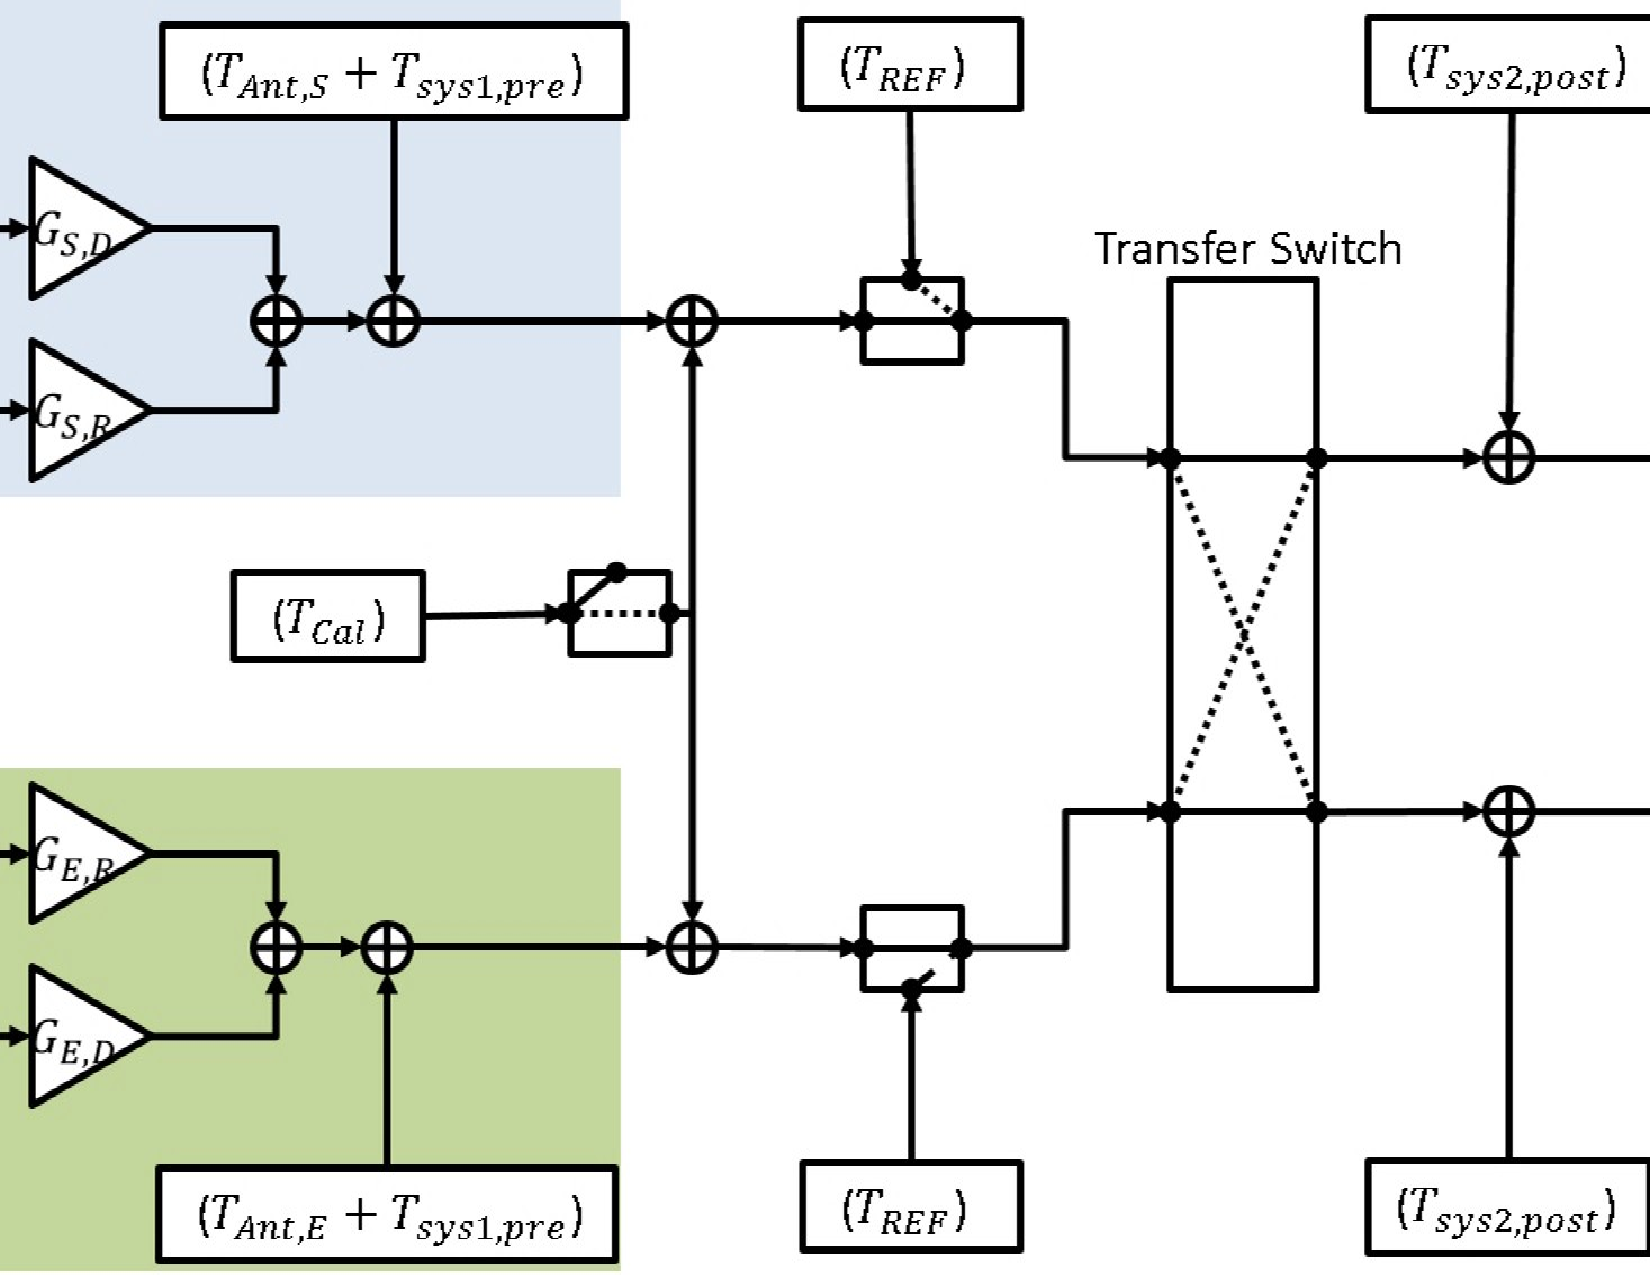
\includegraphics[width=2.5in]{pdf/hardware.pdf}
	\caption{The calibration chain includes antenna swap and noise injection}
	\centering
	\label{fig:Hardware}
\end{figure}
In Figure \ref{fig:Hardware}, $T_{cal}$ is noise temperature of the calibrated noise load, $T_{REF}$ is noise temperature of RF terminator, $T_{sys1,pre}$ and $T_{sys2,pre}$is noise of channel 1 and 2, respectively, prior the transfer switch, $T_{sys1,post}$ and $T_{sys2,post}$is noise of channel 1 and 2, respectively, after the transfer switch, and $T_{ant,S}$ and $T_{ant,E}$is noise of sky-view and earth-view antenna, respectively. There are three modes of calibration chain. The noise power $\sigma^2$ is given by
\begin{equation}
	\sigma^2=\kappa TB
\end{equation}
Where $\kappa$ is the Boltzmen constant, $T$ is noise temperature, and $B$ is bandwidth. The first mode is normal mode which means there is no additional noise in the system, and the correlations $\tilde{R}^n$ in Equation \ref{Eq: R11_reduce}, \ref{Eq: R22_reduce}, and \ref{Eq: R11_reduce} can be rewrote as
\begin{eqnarray}
	\tilde{R}_{11}^n(\tau^s) &&= g^2_{1SD} R_a(\tau^s)e^{j\Delta\omega_e\tau_s}+
G_1(\sigma^2_{Ant,S}+\sigma^2_{sys1,pre} +\sigma^2_{sys1,post}) \delta(\tau^s)                                      
\label{Eq: R11_reduce_norm} \\
	\tilde{R}_{22}^n(\tau^s) &&= g^2_{2ER} R_a(\tau^s)e^{j\Delta\omega_e\tau_s}+
G_2(\sigma^2_{Ant,E}+\sigma^2_{sys2,pre} +\sigma^2_{sys2,post}) \delta(\tau^s)                                       
\label{Eq: R22_reduce_norm} \\
	\tilde{R}_{12}^n(\tau^s) &&= g_{1SD} g_{2ER} R_a(\tau^s-\tau^s_{RD})e^{j\omega_e \tau_{RD}} e^{j\Delta\omega_e\tau_s}  
\label{Eq: R12_reduce_norm}
\end{eqnarray}
Once the transfer switch is activated, the the correlations $\tilde{R}^s$ become
\begin{eqnarray}
\tilde{R}_{11}^s(\tau^s) &&= g^2_{1ER} R_a(\tau^s)e^{j\Delta\omega_e\tau_s}+
G_1(\sigma^2_{Ant,E}+\sigma^2_{sys2,pre} +\sigma^2_{sys1,post}) \delta(\tau^s)                                       
\label{Eq: R22_reduce_swap} \\
\tilde{R}_{22}^s(\tau^s) &&= g^2_{2SD} R_a(\tau^s)e^{j\Delta\omega_e\tau_s}+
G_2(\sigma^2_{Ant,S}+\sigma^2_{sys1,pre} +\sigma^2_{sys2,post}) \delta(\tau^s)                                      
\label{Eq: R11_reduce_swap} \\
	\tilde{R}_{12}^s(\tau^s) &&= g_{1SD} g_{2ER} R_a(\tau^s+\tau^s_{RD})e^{-j\omega_e \tau_{RD}} e^{j\Delta\omega_e\tau_s}  
\label{Eq: R12_reduce_swap}
\end{eqnarray}
When the system injects noise from noise load, the the correlations $\tilde{R}^c$ is changed as
\begin{eqnarray}
	\tilde{R}_{11}^c(\tau^s) &&= g^2_{1SD} R_a(\tau^s)e^{j\Delta\omega_e\tau_s}+
G_1(\sigma^2_{Ant,S}+\sigma^2_{sys1,pre} +\sigma^2_{sys1,post}+\sigma^2_{cal}) \delta(\tau^s)                                      
\label{Eq: R11_reduce_cal} \\
	\tilde{R}_{22}^n(\tau^s) &&= g^2_{2ER} R_a(\tau^s)e^{j\Delta\omega_e\tau_s}+
G_2(\sigma^2_{Ant,E}+\sigma^2_{sys2,pre} +\sigma^2_{sys2,post}+\sigma^2_{cal}) \delta(\tau^s)                                       
\label{Eq: R22_reduce_cal} \\
	\tilde{R}_{12}^n(\tau^s) &&= g_{1SD} g_{2ER} R_a(\tau^s-\tau^s_{RD})e^{j\omega_e \tau_{RD}} e^{j\Delta\omega_e\tau_s}\delta(\tau^s)+
    \sqrt{G_1 G_2}\sigma^2_{cal}\delta(\tau^s)  
\label{Eq: R12_reduce_cal}
\end{eqnarray}The last mode switches the signal sources to reference load in the following equation.
\begin{eqnarray}
	\tilde{R}_{11}^r(\tau^s) &&= G_1(\sigma^2_{REF}+\sigma^2_{sys1,post}) \delta(\tau^s)                                      
\label{Eq: R11_reduce_ref} \\
	\tilde{R}_{22}^r(\tau^s) &&= G_2(\sigma^2_{REF}+\sigma^2_{sys2,post}) \delta(\tau^s)                                
\label{Eq: R22_reduce_ref} \\
	\tilde{R}_{12}^r(\tau^s) &&= 0 
\label{Eq: R12_reduce_ref}
\end{eqnarray}
\section{The injection of noise from noise source and terminator}
The channel gains $G_1$ and $G_2$ are estimated from  $\tilde{R}^n_*$ in Equations \ref{Eq: R11_reduce_norm}-\ref{Eq: R12_reduce_norm} and $\tilde{R}^c_*$ in Equations \ref{Eq: R11_reduce_cal}-\ref{Eq: R12_reduce_cal}, and the noise power from noise load $\sigma^2_{cal}$. The product of channel gain and $\sigma^2_{cal}$ is calculated in
\begin{eqnarray}
	\tilde{R}^c_{11}(0) - \tilde{R}^n_{11}(0)&&= G_1\sigma^2_{cal} \label{Eq: Cal_channel_gain1a} \\
    \tilde{R}^c_{22}(0) - \tilde{R}^n_{22}(0)&&= G_2\sigma^2_{cal} \label{Eq: Cal_channel_gain2a} \\
    \tilde{R}^c_{12}(\tau_{RD}) - \tilde{R}^n_{12}(\tau_{RD})&&= \sqrt{G_1 G_2}\sigma^2_{cal} \label{Eq: Cal_channel_gain12a}
\end{eqnarray}
Once $\sigma^2_{cal}$ is well measured, 
\begin{eqnarray}
	G_1 &&= \frac{\tilde{R}^c_{11}(0) - \tilde{R}^n_{11}(0)}{\sigma^2_{cal}}  \label{Eq: Cal_channel_gain1} \\
    G_2 &&= \frac{\tilde{R}^c_{22}(0) - \tilde{R}^n_{22}(0)}{\sigma^2_{cal}}  \label{Eq: Cal_channel_gain2} \\
    \sqrt{G_1 G_2} &&= \frac{\tilde{R}^c_{12}(\tau_{RD}) - \tilde{R}^n_{12}(\tau_{RD})}{\sigma^2_{cal}}  \label{Eq: Cal_channel_gain12}
\end{eqnarray}

The noise of channel 1 and 2 after the transfer switch are further estimated by substituting $G_1$ and $G_2$ into Equations \ref{Eq: R11_reduce_ref} and \ref{Eq: R22_reduce_ref}. The Equations \ref{Eq: R11_reduce_ref} and \ref{Eq: R22_reduce_ref} are rewrote as
\begin{eqnarray}
	\sigma^2_{sys1,post} &&= \frac{\tilde{R}^r_{11}(0) }{G_1}-\sigma^2_{REF}  \label{Eq: Cal_channel_noise1} \\
    \sigma^2_{sys2,post} &&= \frac{\tilde{R}^r_{22}(0) }{G_2}-\sigma^2_{REF}  \label{Eq: Cal_channel_noise2} 
\end{eqnarray}
\section{Antenna swapping}
The antenna swapping \cite{Alejandro:2013} is used for the estimation of the ratio of channel gain $\frac{G_1}{G_2}$, and it can be measured by the ratio of $\tilde{R}^s$ Equations \ref{Eq: R11_reduce_swap}-\ref{Eq: R12_reduce_swap} and $\tilde{R}^n$Equations \ref{Eq: R11_reduce_norm}-\ref{Eq: R12_reduce_norm}. When the noise of channels are approximately same, the ratio of channel gain is calculated as
\begin{eqnarray}
	\frac{G_1}{G_2} = \frac{\tilde{R}^n_{11}}{\tilde{R}^s_{11}} \\
    \frac{G_1}{G_2} = \frac{\tilde{R}^s_{22}}{\tilde{R}^n_{22}}  \label{Eq: Cal_channel_gain_ratio}
\end{eqnarray}

\section{Conclusion}
The conclusion goes here.





% if have a single appendix:
%\appendix[Proof of the Zonklar Equations]
% or
%\appendix  % for no appendix heading
% do not use \section anymore after \appendix, only \section*
% is possibly needed

% use appendices with more than one appendix
% then use \section to start each appendix
% you must declare a \section before using any
% \subsection or using \label (\appendices by itself
% starts a section numbered zero.)
%


\appendices
\section{Proof of the First Zonklar Equation}
Appendix one text goes here.

% you can choose not to have a title for an appendix
% if you want by leaving the argument blank
\section{}
Appendix two text goes here.


% use section* for acknowledgment
\section*{Acknowledgment}


The authors would like to thank...


% Can use something like this to put references on a page
% by themselves when using endfloat and the captionsoff option.
\ifCLASSOPTIONcaptionsoff
  \newpage
\fi



% trigger a \newpage just before the given reference
% number - used to balance the columns on the last page
% adjust value as needed - may need to be readjusted if
% the document is modified later
%\IEEEtriggeratref{8}
% The "triggered" command can be changed if desired:
%\IEEEtriggercmd{\enlargethispage{-5in}}

% references section

% can use a bibliography generated by BibTeX as a .bbl file
% BibTeX documentation can be easily obtained at:
% http://www.ctan.org/tex-archive/biblio/bibtex/contrib/doc/
% The IEEEtran BibTeX style support page is at:
% http://www.michaelshell.org/tex/ieeetran/bibtex/
%\bibliographystyle{IEEEtran}
% argument is your BibTeX string definitions and bibliography database(s)
%\bibliography{IEEEabrv,../bib/paper}
%
% <OR> manually copy in the resultant .bbl file
% set second argument of \begin to the number of references
% (used to reserve space for the reference number labels box)
\begin{thebibliography}{1}

\bibitem{Ulaby:1981}
F. T. Ulaby, R. K. Moore, and A. K. Fung, Microwave Remote Sensing: From theory to applications: Addison-Wesley Publishing Company, Advanced Book Program/World Science Division, 1981.

\bibitem{Saxton:1986}
K. E. Saxton, W. J. Rawls, J. S. Romberger, and R. I. Papendick, "Estimating Generalized Soil-water Characteristics from Texture1," Soil Sci. Soc. Am. J., vol. 50, pp. 1031-1036, 1986 1986.

\bibitem{Peplinski:1995}
N. R. Peplinski, F. T. Ulaby, and M. C. Dobson, "Dielectric properties of soils in the 0.3-1.3-GHz range," Geoscience and Remote Sensing, IEEE Transactions on, vol. 33, pp. 803-807, 1995.

\bibitem{Peplinski_correct:1995}
N. R. Peplinski, F. T. Ulaby, and M. C. Dobson, "Corrections to "Dielectric Properties of Soils in the 0.3-1.3-GHz Range"," Geoscience and Remote Sensing, IEEE Transactions on, vol. 33, p. 1340, 1995.

\bibitem{Jin:2011}
S. Jin, G. P. Feng, and S. Gleason, "Remote sensing using GNSS signals: Current status and future directions," Advances in Space Research, vol. 47, pp. 1645-1653, 5/17/ 2011.

\bibitem{Zavorotny:2010}
V. U. Zavorotny, K. M. Larson, J. J. Braun, E. E. Small, E. D. Gutmann, and A. L. Bilich, "A Physical Model for GPS Multipath Caused by Land Reflections: Toward Bare Soil Moisture Retrievals," Selected Topics in Applied Earth Observations and Remote Sensing, IEEE Journal of, vol. 3, pp. 100-110, 2010.

\bibitem{Matt:2014}
K. Rautiainen, J. Lemmetyinen, M. Schwank, A. Kontu, C. B. Ménard, C. Mätzler, et al., "Detection of soil freezing from L-band passive microwave observations," Remote Sensing of Environment, vol. 147, pp. 206-218, 5/5/ 2014.

\bibitem{Larson:2008}
K. M. Larson, E. E. Small, E. D. Gutmann, A. L. Bilich, J. J. Braun, and V. U. Zavorotny, "Use of GPS receivers as a soil moisture network for water cycle studies," Geophys. Res. Lett., vol. 35, p. L24405, 2008.

\bibitem{Shah:2011}
R. Shah, J. L. Garrison, and M. S. Grant, "Anisotropy in ocean scattering of bistatic radar using signals of opportunity," in Geoscience and Remote Sensing Symposium (IGARSS), 2011 IEEE International, 2011, pp. 4229-4232.

\bibitem{Kerr:2000}
Y. H. Kerr, J. Font, P. Waldteufel, and M. Berger, "The Soil Moisture and Ocean Salinity Mission - SMOS," in ESA Earth Observation Quarterly, ed, 2000, pp. 18-25.

\bibitem{Wang:2009}
L. Wang and J. J. Qu, "Satellite remote sensing applications for surface soil moisture monitoring: A review," Frontiers of Earth Science in China, vol. 3, pp. 237-247, 2009.

\bibitem{Entekhabi:2010}
D. Entekhabi, E. G. Njoku, P. E. O'Neill, K. H. Kellogg, W. T. Crow, W. N. Edelstein, et al., "The Soil Moisture Active Passive (SMAP) Mission," PROCEEDINGS OF THE IEEE, vol. 98, pp. 704-716, 2010.

\end{thebibliography}

% biography section
% 
% If you have an EPS/PDF photo (graphicx package needed) extra braces are
% needed around the contents of the optional argument to biography to prevent
% the LaTeX parser from getting confused when it sees the complicated
% \includegraphics command within an optional argument. (You could create
% your own custom macro containing the \includegraphics command to make things
% simpler here.)
%\begin{IEEEbiography}[{\includegraphics[width=1in,height=1.25in,clip,keepaspectratio]{mshell}}]{Michael Shell}
% or if you just want to reserve a space for a photo:

\begin{IEEEbiography}{Michael Shell}
Biography text here.
\end{IEEEbiography}

% if you will not have a photo at all:
\begin{IEEEbiographynophoto}{John Doe}
Biography text here.
\end{IEEEbiographynophoto}

% insert where needed to balance the two columns on the last page with
% biographies
%\newpage

\begin{IEEEbiographynophoto}{Jane Doe}
Biography text here.
\end{IEEEbiographynophoto}

% You can push biographies down or up by placing
% a \vfill before or after them. The appropriate
% use of \vfill depends on what kind of text is
% on the last page and whether or not the columns
% are being equalized.

%\vfill

% Can be used to pull up biographies so that the bottom of the last one
% is flush with the other column.
%\enlargethispage{-5in}



% that's all folks
\end{document}